\section{Introduction and motivation}

Data visualisation is an essential component of modern data science and science
communication. The power of data visualisation as a communicative tool means it
is also open to both misinterpretation and misuse: patterns in raw data can be
obscured, statistical assumptions hidden, and effect sizes misrepresented
\cite{weissgerber15}. These concerns can be addressed in part through improved
statistical practices and novel plot and chart designs \cite{allen19}, but also
by making visualisations themselves more open and explorable
\cite{dragicevic19}.

One well-established technique for explorability is \emph{linked brushing}
\cite{fisherkeller75,becker87,buja91}, which allows the user to explore
interactively how a visualisation relates to other concurrent visualisations of
the same underlying data. For example, geoscientists often work with multiple
layered views. To show how these are related, spatial analytics applications
like GeoDa \cite{anselin06} can automatically select the relevant part of one
view as the user changes the selection in a related view, say a choropleth map.
Such linking is an important navigational tool, allowing the user to switch
contexts in one view and have related views synchronise automatically. With
complex multivariate data, linking can be an essential sense-making aid, helping
the user intuit relationships in the data and grasp what the views themselves
represent \cite{he18}.

However, the linked brushing feature is usually only available if it was
specifically anticipated by the application or library developer. If the data
analyst uses custom libraries or wants other views or visual attributes linked
that the developer did not consider, they are out of luck. For example, the
Bokeh library for Python \cite{jolly18} provides linked brushing automatically
whenever the glyph renderers for two different charts share a data source. This
makes it easy to for example create a histogram which is linked to a
scatterplot.

[Moroever, code/data..debugging..transparency/reproducibility]

\begin{figure}[H]
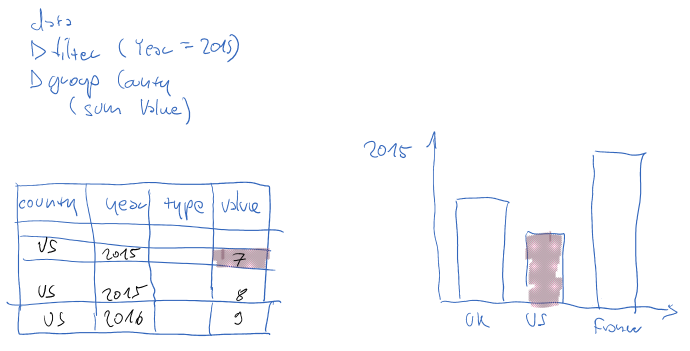
\includegraphics[scale=0.35]{image/chart-fwd}
\caption{Forward linking from code and data to visualisation}
\end{figure}

In this short paper, we present a framework for authoring visualisations where
support for linking is built in, making this powerful comprehension feature
automatic. Moreover, [between data, code, and visualisations.]
